\section{Overview and Implementation Plan}
In this section we describe how our system needs to be implemented and the actual integration of all its parts: generally, we will follow the bottom-up strategy to implement the single parts of the application (since we structured it as an amalgamation of microservices), this approach will help us in the testing phase because it will allow us to individually test all of the microservices in an isolated enviroment thanks to the creation of individual drivers for each microservice. Also, it allows us to follow a stub-free implementation making the workflow simple and since we have different microservices it is possible to develop them in parallel with more developers at work at the same time, promoting a more diverse testing.

\subsection{Features Identification}

In this subsection, we identify and describe the main features that need to be developed to build a fully functional system. These features have been prioritized to ensure a smooth development workflow and integration.

\begin{itemize}
    \item \textbf{[F1] Authentication Features}:  
    Includes user registration, login, and logout functionalities. These features form the foundation of the system, enabling secure user access and identity management. They will be implemented first due to their critical role in enabling all other features.

    \item \textbf{[F2] Creation Features}:  
    Encompasses the creation of key entities such as Trips, Paths, and Bike-related data entries. These features allow users to add new data to the system and are prerequisites for view and search functionalities.

    \item \textbf{[F3] View Features}:  
    Allows users to visualize Trips, Paths, Profiles, and other relevant data. These features depend on the creation features to display meaningful content.

    \item \textbf{[F4] Search Features}:  
    Enables users to search for bike paths, trips, and user profiles based on various criteria. These features require both creation and view features to be functional.

    \item \textbf{[F5] Join Features}:  
    Includes operations for users to participate in groups or collaborative activities related to bike paths or trips. Requires view and creation features for proper operation.

    \item \textbf{[F6] Evaluation Features}:  
    Comprises both manual and automated evaluation of trip data, sensor accuracy, and path quality. These features integrate external tools and require extensive data processing capabilities.

    \item \textbf{[F7] Notification Features}:  
    Handles system-generated notifications to users regarding path updates, trip confirmations, and other important events. This feature relies on the successful implementation of most other features and will be implemented last.
\end{itemize}

\section{Integration Strategy}
In order to develop our managers we will firstly need a working instance of a DBMS (that is to be intended the real one that we will be using when going into production or a local instance saved inside the same machine where we are implementing everything, for testing purposes) and a rudimental version of the client-side app (a stub can also work out, the important thing is that we need to see the messages that will be sent from the notification manager to the view): once those two elements are present and working, it is possible to start developing the first parts of our application.

\subsection{Query Manager and Notification Manager}
The first two components to be implemented and tested are the query manager and the notification manager: since they're completely indipendent from one to another it is also possible to develop them in parallel. 
The query manager contains all the queries to be made at the DBMS: it is not only a crucial component to test since every manager will eventually use it but also a difficult one, since the only way to actually test the effectiveness of the queries is to actually execute them. It is preferred to start with a mock schema with false informations so that it is verified that the queries actually work.
The notification manager is the equivalent of the query manager for the front-end of our application: it is easier to test since In testing phase it can also be used as a useful tool to allow us to see what the user sees in the client-side view.
\begin{figure}[H]
	\centering
	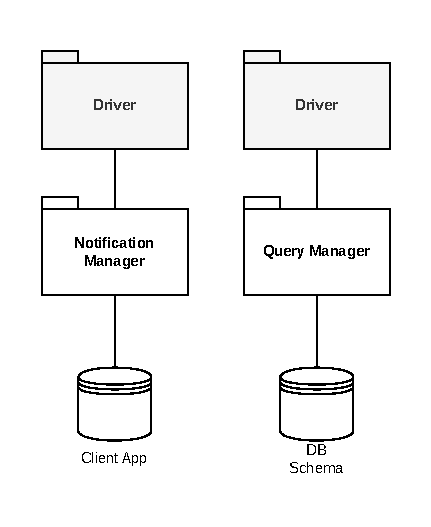
\includegraphics[width=0.7\textwidth]{Test Diagrams/5-queryNotificationManagerTesting.pdf}
	\caption{Query Manager and Notification Manager testing}
\end{figure}

\subsection{Storage, Search, Profile, Look Publish, Recording, Merge and Authentication Managers}
Since we now have the two main components of our system that drive the main front-end and back-end communication, it is possible to implement in parallel the principal managers that make up the main logic of the application: this also allows for last-minute additions if some added functionalities are needed (with relative managers).
\begin{figure}[H]
	\centering
	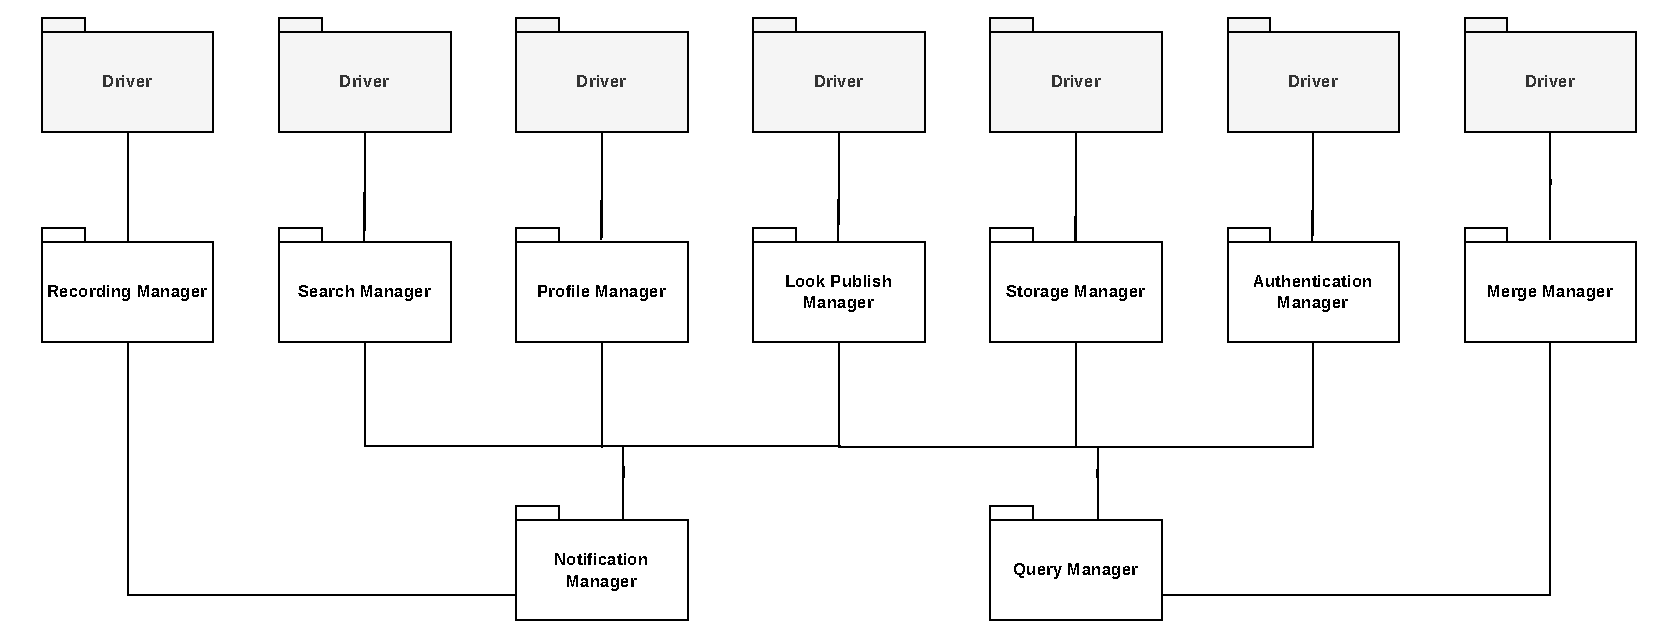
\includegraphics[width=\textwidth]{Test Diagrams/5-parallelManagerTesting.pdf}
	\caption{Parallel Managers testing}
\end{figure}
Note: for the Recording Manager, which has two submodules for automated and manual recording of trips, it is necessary to develop the common module first and then the specific modules.

\subsection{Dashboard Manager}
Finally, the dashboard manager will connect all the managers and use the dashboard interface to display all informations correctly: the only logical thing to test is the correct order of display of every content illustrated by the app.
\begin{figure}[H]
	\centering
	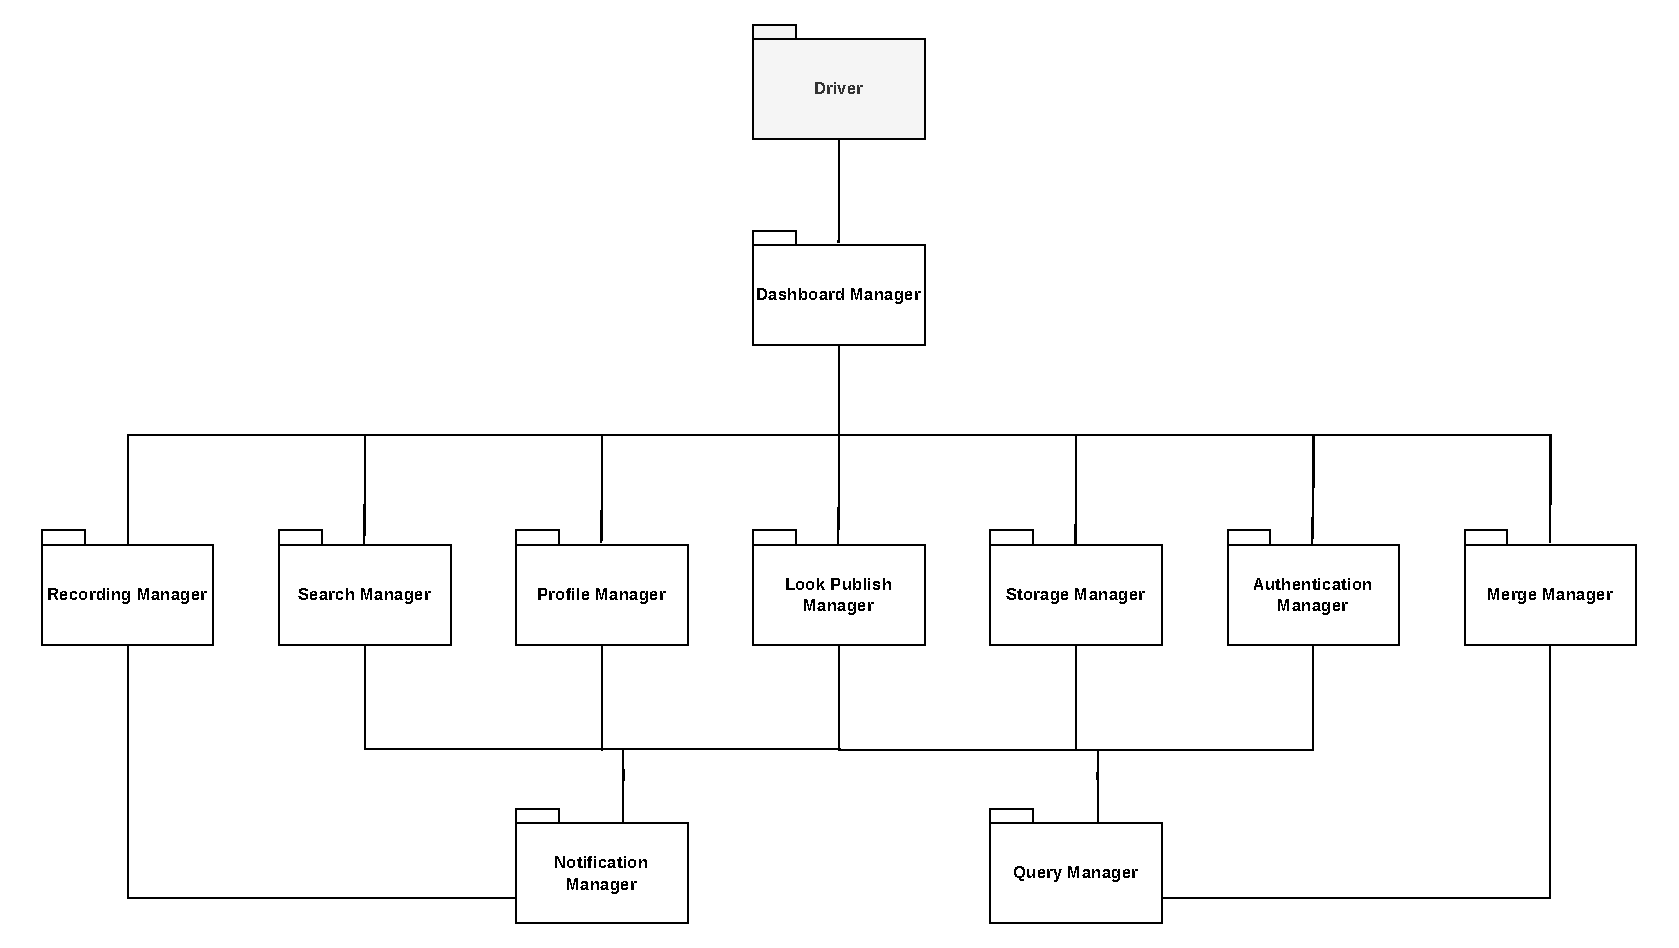
\includegraphics[width=\textwidth]{Test Diagrams/5-dashboardManagerTesting.pdf }
	\caption{Dashboard Manager testing}
\end{figure}


\subsection{System Testing Strategy}

A comprehensive testing strategy is essential to ensure the system’s reliability, performance, and usability. The testing will be performed incrementally as modules are developed and integrated, with the following types of tests applied:

\begin{itemize}
    \item \textbf{Functional Testing}:  
    Verify that each feature behaves according to the requirements specified in the RASD document. Functional tests will cover user workflows, feature interactions, and compliance with business rules.

    \item \textbf{Load Testing}:  
    Assess the system’s ability to handle expected volumes of data and user interactions. This includes testing for memory leaks, buffer overflows, and resource management under continuous load.

    \item \textbf{Performance Testing}:  
    Identify bottlenecks and ensure the system maintains responsive behavior under heavy workload conditions. Performance metrics such as response time, throughput, and resource utilization will be monitored.

    \item \textbf{Stress Testing}:  
    Test the system’s robustness by simulating extreme conditions, such as a high number of concurrent users or limited computational resources, to observe recovery behavior and failure handling.

    \item \textbf{User Interface Testing}:  
    Ensure the application is usable and accessible across different devices, screen sizes, and browsers. Testing will include responsiveness, navigation, and compliance with accessibility standards for both Educators and Students.

\end{itemize}